\documentclass{article}

\usepackage[english]{babel}

\usepackage[letterpaper,top=2cm,bottom=2cm,left=3cm,right=3cm,marginparwidth=1.75cm]{geometry}

% Useful packages
\usepackage{amsmath}
\usepackage{amssymb}
\usepackage{xcolor}
\usepackage{graphicx}
\usepackage{mathtools}
\usepackage{framed}
\usepackage{tikz}
\usepackage[colorlinks=true, allcolors=blue]{hyperref}
\usepackage{xcolor}
\usepackage{colortbl}
\usepackage{booktabs}
\usepackage{tikz}
\usepackage{tcolorbox}
\usepackage{amsthm}
\usetikzlibrary{positioning, arrows.meta}

\theoremstyle{definition}
\newtheorem{exmp}{Example}[section]

\definecolor{sigblue}{RGB}{214,228,247}
\definecolor{siggreen}{RGB}{208,235,203}
\definecolor{sigyellow}{RGB}{255,245,200}

\newcommand{\Fp}{\mathbb F_p}
\newcommand{\Fq}{\mathbb F_q}
\newcommand{\offdest}{\text{off}_{\text{dest}}}
\newcommand{\offopzero}{\text{off}_{\text{op0}}}
\newcommand{\offopone}{\text{off}_{\text{op1}}}
\newcommand*{\logeq}{\ratio\Leftrightarrow}
\newcommand{\nextmle}{\overset{\scriptscriptstyle\wedge}{\textsf{next}}}

\newtheorem{lemma}{Lemma}
\newtheorem{theorem}{Theorem}

\title{LeanVM}
\author{draft 0.8.0}
\date{}
\begin{document}

\maketitle

\tableofcontents
\newpage

\section{Introduction}
Ethereum's cryptography currently relies on elliptic curves, which are known to be vulnerable to quantum computers \cite{shor}.

LeanVM is a verifiable Virtual Machine (also called zkVM for "zero knowledge VM"). It uses a minimal ISA (Intruction Set Architecture) inspired by Cairo \cite{cairo}.
\begin{itemize}
    \item It's hash-based (WHIR \cite{whir}): plausibly post-quantum, conceptually simple
    \item It's multilinear: the trace is committed as a single multilinear polynomial (reducing proof size), and constraints are proven via sumcheck \cite{sumcheck}
    \item It uses the Poseidon \cite{poseidon1} permutation as a snark-friendly hashing primitive
\end{itemize}

\section{Use-cases}

LeanVM is optimized to provide a post-quantum alternative for each of the three layers of Ethereum:

\subsection{Consensus Layer}
\begin{itemize}
    \item \textbf{Currently (pre-quantum):} BLS \cite{bls}: lightweight signatures of 96 bytes, with native support for aggregation.
    \item \textbf{With LeanVM (post-quantum):} Replace BLS by XMSS over poseidon \cite{ethereum_signatures} (leanXMSS). Aggregate those signatures using leanVM. Already aggregated signatures can be further merged, via recursion. XMSS is a statefull signature scheme, but Ethereum's slot can be used a nonce (double signing is already prevented).
\end{itemize}

See \ref{sec:signature-aggregation} for more details.

\subsection{Execution Layer}
\begin{itemize}
    \item \textbf{Currently (pre-quantum):} ECDSA \cite{ecdsa}
    \item \textbf{With LeanVM (post-quantum):} Replace ECDSA by a variant of SPHINCS+ \cite{sphincs_plus} over poseidon (leanSPHINCS). Aggregate all the signatures from one block using leanVM.
\end{itemize}

See \ref{sec:signature-aggregation} for more details.

\subsection{Data Availability Layer}

\begin{itemize}
    \item \textbf{Currently (pre-quantum):} KZG polynomial commitment scheme \cite{kzg}
    \item \textbf{With LeanVM (post-quantum):} Read-Solomon encode and Merkle-commit the codeword, for each blob. Prove the claimed Merkle Root was correctly computed using leanVM.
\end{itemize}

\section{Preliminaries}

\subsection{Notations}

\begin{itemize}
    \item $[a, b] = \{a, a + 1, \ldots, b\}$
    \item $[a, b) = \{a, a + 1, \ldots, b-1\}$    \item $\hat{eq}(x, y) = x y + (1 - x)(1 - y)$
    \item $\mathsf{embed}(x_1, x_2, x_3, x_4, x_5)$ is the extension field element built from 5 base field elements: $x_1 + x_2 X + x_3 X^2 + x_4 X^3 + x_5 X^4$, using $X^5 + X^2 - 1$ as the irreducible polynomial defining the extension.
    \item Given a number of bits $n > 0$, and an $n$-bit iteger $x$, we denote by $[x]_{01}$ its big-endian bit-decomposion in $n$ boolean values. For example, $[14]_{01} = (1, 1, 1, 0)$
    
    \item $M$ is the size of the (read-only) memory, which is a power of 2.
    \item $\textbf{m}[i]$ is the value of the memory at index $i$. It is defined only for $0 \leq i < M$; any out-of-bound access ($i \geq M$) makes the execution \emph{invalid}. More generally, any vector of field elements $v$ is indexed starting at $v[0], v[1], \dots$
    \item $\textbf{m}[i..j]$ is the memory slice $(\textbf{m}[i], \textbf{m}[i+1], \ldots, \textbf{m}[j-1])$.
    \item $||$ denotes concatenation of slices.
    \item $0_k$ denotes the all-zero vector of length $k$, for $k \geq 0$.
    \item $x \overset{\$}{\leftarrow} S$ means $x$ is sampled uniformly at random from the finite set $S$.
\end{itemize}

\subsection{Definitions}

\subsubsection{Multilinear Extension (MLE)}

For a vector of field elements $v \in \mathbb F^{2^n}$ (for some $n \geq 0$), the Multilinear Extension (MLE) of $v$, denoted by $\hat{v}$, is the unique multilinear polynomial in $\mathbb F[X_1, \dots, X_n]$, in $n$ variables, such that: $\forall i \in [0, 2^n), v[i] = \hat{v}([i]_{01})$

Throughout, $v$ denotes a vector and $\hat{v}$ its MLE.

\vspace{5mm}

\subsubsection{$\Fp$-valued multiset}\label{sec:fp-multiset}

An \emph{$\Fp$-valued multiset} over a set $X$ is a function $M : X \to \Fp$ assigning a multiplicity in $\Fp$ to each element of $X$. Its \emph{support} is $\mathrm{supp}(M) = \{x \in X : M(x) \neq 0\}$, and $M$ is the \emph{zero multiset} when $\mathrm{supp}(M) = \emptyset$.

\vspace{5mm}

\subsubsection{Inner Product Commitment Scheme}\label{sec:inner_product_PCS}

An \textit{Inner Product Commitment Scheme} is an interractive protocol where a prover commits to a vector of field elements $v \in \Fp^{2^n}$ (for some $n \geq 0$), and later convince a verifier of the evaluation of $\sum_{i = 0}^{2^n} v[i] \cdot x[i]$ for some arbitrary vector $x \in \Fq^{2^n}$, assuming the verifier is able to evaluate the MLE of $x$.

WHIR \cite{whir} is an example of Inner Product Commitment Scheme.


\vspace{5mm}

\subsubsection{Shifted polynomial}\label{sec:shifts}

Given a vector $v \in \Fp^{2^n}$, we define $\mathsf{shift}(v)  \in \Fp^{2^n}$ by $\mathsf{shift}(v)[2^n - 1] = v[2^n - 1]$ and:

$$
\forall i [0, 2^n - 1), \mathsf{shift}(v)[i] = v[i + 1]
$$

\subsubsection{The next multilinear}\label{sec:next-mle}

For $n \geq 0$, identify each $x \in \{0,1\}^n$ with the integer it encodes in big-endian. We define $\nextmle$ as the multilinear polynomial in $2n$ variables whose values on the boolean hypercube are
\[
\nextmle(x, y) =
\begin{cases}
1 & \text{if } y = x + 1, \\
1 & \text{if } x = y = 2^n - 1, \\
0 & \text{otherwise},
\end{cases}
\qquad x, y \in \{0,1\}^n .
\]

$\nextmle$ can be efficiently evaluated:
\[
\nextmle((x_0, \ldots, x_{n-1}), (y_0, \ldots, y_{n-1})) \;=\; \prod_{j=0}^{n-1} x_j\, y_j \;+\; \sum_{k=0}^{n-1} \Bigg( \prod_{j<k} \hat{eq}(x_j, y_j) \Bigg)\, (1 - x_k)\, y_k \, \Bigg( \prod_{j>k} x_j\, (1 - y_j) \Bigg) .
\]
The leading product is the wrap-around case $x = y = 2^n - 1$. The $k$-th term of the sum is the case $y = x + 1$ with the carry stopping at bit $k$: the high bits ($j < k$) are unchanged, bit $k$ flips $0 \to 1$, and the low bits ($j > k$) flip $1 \to 0$.

The polynomial $\nextmle$ enables sumcheck-based evaluation of shifted MLEs \ref{sec:shifts}: for every $v \in \Fp^{2^n}$,
\[
\overset{\scriptscriptstyle\wedge}{\textsf{shift}(v)}(x) \;=\; \sum_{y \in \{0,1\}^n} \nextmle(x, y)\; \hat{v}(y) ,
\]

\subsection{Lemmas}

\subsubsection{Schwartz-Zippel}

\begin{lemma}[Schwartz-Zippel]\label{lem:sz}
Let $P \in \Fq[X_1, \ldots, X_n]$ be a non-zero polynomial of total degree $d$. Then
\[
\Pr_{\vec\beta \,\overset{\$}{\leftarrow}\, \Fq^n}\big[P(\vec\beta) = 0\big] \;\leq\; \frac{d}{q}.
\]
\end{lemma}
\begin{proof}
By induction on $n$. For $n = 1$, $P$ is a non-zero univariate polynomial of degree $d$, hence has at most $d$ roots in $\Fq$, so $\Pr_\beta[P(\beta) = 0] \leq d/q$.

For $n \geq 2$, write $P$ as a polynomial in $X_n$ with coefficients in $\Fq[X_1, \ldots, X_{n-1}]$:
\[
P(X_1, \ldots, X_n) \;=\; \sum_{k=0}^{d} X_n^k \, Q_k(X_1, \ldots, X_{n-1}),
\]
and let $k^\star = \max\{k : Q_k \neq 0\}$. Then $Q_{k^\star}$ is a non-zero polynomial in $n-1$ variables of total degree at most $d - k^\star$. By the induction hypothesis, $\Pr_{\vec\beta_{<n}}[Q_{k^\star}(\vec\beta_{<n}) = 0] \leq (d - k^\star)/q$. Conditioned on $Q_{k^\star}(\vec\beta_{<n}) \neq 0$, the polynomial $X_n \mapsto P(\vec\beta_{<n}, X_n)$ has degree exactly $k^\star$, hence at most $k^\star$ roots in $\Fq$, so $\Pr_{\beta_n}[P(\vec\beta) = 0 \mid Q_{k^\star}(\vec\beta_{<n}) \neq 0] \leq k^\star/q$. A union bound gives $\Pr_{\vec\beta}[P(\vec\beta) = 0] \leq d/q$.
\end{proof}

A useful consequence: a non-zero multilinear polynomial in $n$ variables has total degree $\leq n$, so it vanishes at a uniform $\vec\beta \in \Fq^n$ with probability at most $n/q$. 

\subsection{Constants}

\begin{center}
\begin{tabular}{lll}
\toprule
Symbol & Value & Description \\
\midrule
$M_\text{min}$ & $2^{16}$ & minimum size of the memory \\
$M_\text{max}$ & $2^{26}$ & maximum size of the memory \\
$M_\text{public}$ & variable, power of $2$, $\leq M$ & size of the public memory \\
$h^{min}$ & 8 & log2 of the minimum number of rows in any table \\
$h^{max}_\text{execution}$ & 24 & log2 of the maximum of rows in the \texttt{execution} table \\
$h^{max}_\text{poseidon}$ & 21 & log2 of the maximum of rows in the \texttt{poseidon} table \\
$h^{max}_\text{extension}$ & 21 & log2 of the maximum of rows in the \texttt{extension} table \\
$\textsf{bus\_width}$ & 16 & number of field elements in the bus (see Section~\ref{sec:Bus: interractions between table via logup-GKR}) \\
$\ell$ & 4 & $\log_2(\textsf{bus\_width})$ \\
$\textsf{memory\_sep}$ & 1 & domain separator of memory interactions \\
$\textsf{bytecode\_sep}$ & 2 & domain separator of bytecode interactions \\
\bottomrule
\end{tabular}
\end{center}

\section{VM specification}
\subsection{Field}

The base field is $\Fp$, with $p = 2^{31} - 2^{24} + 1$ (KoalaBear prime). The extension field is $\Fq$, with $q = p^5$ (degree 5 extension).


\subsection{Poseidon specification}

We use the Poseidon \cite{poseidon1} permutation, over a state of 16 (base) field elements: 

$$\texttt{POSEIDON}^\pi: \Fp^{16} \to \Fp^{16}$$

The MDS matrix is circulant, with first row $[1, 3, 13, 22, 67, 2, 15, 63, 101, 1, 2, 17, 11, 1, 51, 1]$.

There are $N_\text{full} / 2 = 4$ initial full rounds, $N_\text{partial} = 20$ partial rounds, and $N_\text{full} / 2 = 4$ final full rounds.

TODO explain how round constants were generated.

\vspace{3mm}

Poseidon can be used in "compression" mode (feed-forward):

\begin{align*}
\texttt{POSEIDON}^C: \Fp^{16} &\to \Fp^{8} \\
x &\mapsto (\texttt{POSEIDON}^\pi(x) + x)[0..8]
\end{align*}

where $+$ represents field coordinate-wise addition, and $[0..8]$ represents the first 8 elements of the result.


\subsection{Memory}

We use a read-only memory (also called write-once memory). Each memory word is a base field element. The memory is a 1D array of $M$ words. The size of the memory, is attached to each execution of the VM. Valid sizes are $M_\text{min} \leq M \leq M_\text{max}$, with $M_\text{min} = 2^{16}$ and $M_\text{max} = 2^{26}$. The first $M_{\text{public}} \leq M$ memory cells hold the "public input", which informally represents the part of the memory "controlled" by the verifier of an execution proof. Both $M$ and $M_{\text{public}}$ must be powers of 2.

\subsection{Bytecode}

The bytecode is also read-only, and also has a power of two size. It lives in a separate region than the memory (Harvard architecture). Both prover and verifier are expected to have access to the bytecode. Each bytecode specifies the size of the public input $M_{\text{public}}$. For a bytecode of size $2^b$, a valid execution should start at $\textbf{pc} = 0$, and end at $\textbf{pc} = 2^b - 1$. In practice, it is suggested to use for the last instruction (at index $2^b - 1$) a \texttt{JUMP} (\ref{sec:jump}) that inconditionally jumps to itself (for padding reasons within the snark). The minimal size for a bytecode is $2^{h^{min}}$.

\subsection{Registers}

The VM uses two registers \textbf{pc} and \textbf{fp} that fully describes its state. Everything else (memory and bytecode) is read-only.

\begin{itemize}
    \item \textbf{pc}: program counter, points to the current instruction
    \item \textbf{fp}: frame pointer, points to the start of the current "frame" in memory
\end{itemize}

 Except for JUMP, every instruction updates them by $\textbf{pc} \gets \textbf{pc} + 1$ and $\textbf{fp} \gets \textbf{fp}$.



\subsection{Addressing modes}

Most of the operands usually come in pair $(x^\text{addr}, x)$:
\begin{itemize}
    \item one \textit{addressing mode} $x^\text{addr} \in \{\,\texttt{imm},\ \texttt{mem},\ \texttt{fp\_rel}\,\}$
    \item one \textit{value} $x \in \Fp$
\end{itemize}

At runtime, it resolves to:
\[
\mathsf{val}(x^\text{addr}, x) =
\begin{cases}
x & \text{if } x^\text{addr} = \texttt{imm} \quad \text{(immediate)} \\
\textbf{m}[\textbf{fp} + x] & \text{if } x^\text{addr} = \texttt{mem} \quad \text{(memory)} \\
\textbf{fp} + x & \text{if } x^\text{addr} = \texttt{fp\_rel} \quad \text{(fp-relative)}
\end{cases}
\]
\subsection{Instruction Set Architecture}

The instruction set comprises 4 \emph{core instructions} (ADD, MUL, DEREF, JUMP) and 2 \emph{precompiles} (POSEIDON\_OP, EXTENSION\_OP).




\subsubsection{ADD}

An addition over the base field $\Fp$.

\[
\texttt{ADD}[\;\alpha^\text{addr},\, \alpha,\;\; \beta^\text{addr},\, \beta,\;\; \gamma^\text{addr},\, \gamma\;]
\]

\textbf{Operands:}
\begin{itemize}
    \item $\alpha, \beta, \gamma \in \Fp$
    \item $\alpha^\text{addr}, \beta^\text{addr} \in \{\texttt{imm}, \texttt{mem}\}$
    \item $\gamma^\text{addr} \in \{\texttt{imm}, \texttt{mem}, \texttt{fp\_rel}\}$
\end{itemize}

\textbf{Semantics.} Write $a = \mathsf{val}(\alpha^\text{addr}, \alpha)$, $b = \mathsf{val}(\beta^\text{addr}, \beta)$, $c = \mathsf{val}(\gamma^\text{addr}, \gamma)$.
\[
a + c = b
\]

\subsubsection{MUL}

A multiplication over the base field $\Fp$.

\[
\texttt{MUL}[\;\alpha^\text{addr},\, \alpha,\;\; \beta^\text{addr},\, \beta,\;\; \gamma^\text{addr},\, \gamma\;]
\]

Same operands as \texttt{ADD}. Reusing the notations above, the semantics is
\[
a \cdot c = b
\]



\subsubsection{DEREF}

A pointer dereference: accesses memory at an address read from another memory cell.

\[
\texttt{DEREF}[\;\alpha,\;\; \beta,\;\; \gamma^\text{addr},\, \gamma\;]
\]

\textbf{Operands:}
\begin{itemize}
    \item $\alpha, \beta, \gamma \in \Fp$
    \item $\gamma^\text{addr} \in \{\texttt{imm}, \texttt{mem}, \texttt{fp\_rel}\}$
\end{itemize}

\textbf{Semantics:}
\[
\textbf{m}\big[\;\textbf{m}[\textbf{fp} + \alpha] + \beta\;\big] \;=\; \mathsf{val}(\gamma^\text{addr}, \gamma).
\]

\subsubsection{JUMP} \label{sec:jump}

A conditional jump.

\[
\texttt{JUMP}[\;\alpha^\text{addr},\, \alpha,\;\; \beta^\text{addr},\, \beta,\;\; \gamma^\text{addr},\, \gamma\;]
\]

\textbf{Operands:}
\begin{itemize}
    \item $\alpha, \beta, \gamma \in \Fp$
    \item $\alpha^\text{addr}, \beta^\text{addr} \in \{\texttt{imm}, \texttt{mem}\}$
    \item $\gamma^\text{addr} \in \{\texttt{imm}, \texttt{mem}, \texttt{fp\_rel}\}$
\end{itemize}

\textbf{Semantics:} Write $\text{cond} = \mathsf{val}(\alpha^\text{addr}, \alpha)$, $\text{updated\_pc} = \mathsf{val}(\beta^\text{addr}, \beta)$, and $\text{updated\_fp} = \mathsf{val}(\gamma^\text{addr}, \gamma)$. The condition is constrained to be boolean, $\text{cond} \in \{0, 1\}$, and the registers are updated by
\[
(\textbf{pc}, \textbf{fp}) \;\gets\;
\begin{cases}
(\,\text{updated\_pc},\; \text{updated\_fp}\,) & \text{if } \text{cond} = 1 \\[2mm]
(\,\textbf{pc} + 1,\; \textbf{fp}\,) & \text{if } \text{cond} = 0
\end{cases}
\]


\subsubsection{POSEIDON\_OP}

A precompile to compute Poseidon in permuation or compression mode.

\[
\texttt{POSEIDON\_OP}[\;\alpha^\text{addr},\, \alpha,\;\; \beta^\text{addr},\, \beta,\;\; \gamma^\text{addr},\, \gamma,\;\; \texttt{permute},\;\; \texttt{half},\;\; \delta\;]
\]

\textbf{Operands:}
\begin{itemize}
    \item $\alpha, \beta, \gamma \in \Fp$
    \item $\alpha^\text{addr}, \beta^\text{addr}, \gamma^\text{addr} \in \{\texttt{imm}, \texttt{mem}, \texttt{fp\_rel}\}$, with $\alpha^\text{addr} = \texttt{fp\_rel} \Leftrightarrow \beta^\text{addr} = \texttt{fp\_rel}$
    \item $\texttt{permute}, \texttt{half} \in \{0, 1\}$,  $\delta \in \Fp \cup \{\bot\}$, with constraint: $\texttt{permute} = 1 \Rightarrow (\texttt{half}, \delta) = (0, \bot)$ 
\end{itemize}

\textbf{Semantics:} Define the pointers $a = \mathsf{val}(\alpha^\text{addr}, \alpha)$, $b = \mathsf{val}(\beta^\text{addr}, \beta)$, $c = \mathsf{val}(\gamma^\text{addr}, \gamma)$.

\textbf{Input.} The $16$-element input $x = L \,||\, R \in \Fp^{16}$ is built from a left half $L$ and a right half $R$:
\[
L =
\begin{cases}
\textbf{m}[a .. a + 8] & \text{if } \delta = \bot \\[1mm]
\textbf{m}[\delta .. \delta + 4] \;||\; \textbf{m}[a .. a + 4] & \text{if } \delta \neq \bot
\end{cases}
\qquad
R = \textbf{m}[b .. b + 8].
\]

\textbf{Output.}
\[
\begin{cases}
\textbf{m}[c .. c + 16] = \texttt{POSEIDON}^\pi(x) & \text{if } \texttt{permute} = 1 \\[1mm]
\textbf{m}[c .. c + 8] = \texttt{POSEIDON}^C(x) & \text{if } \texttt{permute} = 0,\; \texttt{half} = 0 \\[1mm]
\textbf{m}[c .. c + 4] = \texttt{POSEIDON}^C(x)[0..4] & \text{if } \texttt{permute} = 0,\; \texttt{half} = 1
\end{cases}
\]


\subsubsection{EXTENSION\_OP}\label{extension_op_instruction}

A precompile to compute various operations in the extension field, usefull for recursion.


\[
\texttt{EXTENSION\_OP}[\;\alpha^\text{addr},\, \alpha,\;\; \beta^\text{addr},\, \beta,\;\; \gamma^\text{addr},\, \gamma,\;\; \texttt{op},\;\; \texttt{be},\;\; N\;]
\]


\textbf{Operands:}
\begin{itemize}
    \item $\alpha, \beta, \gamma \in \Fp$
    \item $\alpha^\text{addr}, \beta^\text{addr}, \gamma^\text{addr} \in \{\texttt{imm}, \texttt{mem}, \texttt{fp\_rel}\}$, with $\alpha^\text{addr} = \texttt{fp\_rel} \Leftrightarrow \beta^\text{addr} = \texttt{fp\_rel}$
    \item $\texttt{op} \in \{\textsc{add}, \textsc{dot\_product}, \textsc{eq}\}$, $\texttt{be} \in \{0, 1\}$
    \item $N \geq 1$
\end{itemize}

\textbf{Semantics:} Define the pointers $a = \mathsf{val}(\alpha^\text{addr}, \alpha)$, $b = \mathsf{val}(\beta^\text{addr}, \beta)$, $c = \mathsf{val}(\gamma^\text{addr}, \gamma)$.

\textbf{Input.} For each $i \in [0, N)$, define
$
b_i = \mathsf{embed}\big(\textbf{m}[b + 5i \,..\, b + 5i + 5]\big) \in \Fq,
$
and:
\[
a_i =
\begin{cases}
\textbf{m}[a + i] \in \Fp & \text{if } \texttt{be} = 1 \quad \text{(base-extension)} \\[1mm]
\mathsf{embed}\big(\textbf{m}[a + 5i \,..\, a + 5(i + 1)]\big) \in \Fq & \text{if } \texttt{be} = 0 \quad \text{(extension-extension)}
\end{cases}
\]

\textbf{Output.}
\[
\mathsf{embed}\big(\textbf{m}[c \,..\, c + 5]\big) =
\begin{cases}
\sum_{i=0}^{N-1} (a_i + b_i) & \text{if } \texttt{op} = \textsc{add} \\[1mm]
\sum_{i=0}^{N-1} a_i \cdot b_i & \text{if } \texttt{op} = \textsc{dot\_product} \\[1mm]
\prod_{i=0}^{N-1} \hat{eq}(a_i, b_i) & \text{if } \texttt{op} = \textsc{eq}
\end{cases}
\]

\subsection{Example: Fibonacci Program}

The following program takes two base field elements $(n, r)$ as public input, and proves that the $n$-th Fibonacci number, reduced modulo $p$, equals $r$.

\begin{framed}
\small
\noindent
\begin{minipage}[t]{0.48\textwidth}
\begin{verbatim}
[public input size]  2

[program]
   0: ADD[imm, 0,  imm, 0,  mem, 2]
   1: DEREF[2,  0,  mem, 3]
   2: ADD[imm, 1,  mem, 4,  mem, 3]
   3: DEREF[5,  0,  imm, 1]
   4: DEREF[5,  1,  imm, 1]
   5: ADD[imm, 1,  mem, 3,  mem, 6]
   6: DEREF[7,  0,  imm, 34]
   7: DEREF[7,  1,  fp_rel, 0]
   8: DEREF[7,  2,  imm, 0]
   9: DEREF[7,  3,  mem, 5]
  10: DEREF[7,  4,  mem, 3]
  11: DEREF[7,  5,  mem, 6]
  12: JUMP[imm, 1,  imm, 13,  mem, 7]
  13: ADD[mem, 6,  mem, 2,  mem, 5]
  14: MUL[mem, 6,  mem, 8,  mem, 7]
  15: ADD[mem, 9,  imm, 1,  mem, 8]
  16: MUL[mem, 9,  imm, 0,  mem, 6]
  17: JUMP[mem, 8,  imm, 19,  fp_rel, 0]
  18: JUMP[imm, 1,  imm, 32,  fp_rel, 0]
  19: ADD[mem, 3,  mem, 10,  mem, 2]
  20: DEREF[10,  0,  mem, 11]
  21: DEREF[10,  1,  mem, 12]
\end{verbatim}
\end{minipage}
\hfill
\begin{minipage}[t]{0.48\textwidth}
\begin{verbatim}
  22: ADD[mem, 11,  mem, 13,  mem, 12]
  23: DEREF[10,  2,  mem, 13]
  24: ADD[imm, 1,  mem, 14,  mem, 2]
  25: DEREF[15,  0,  mem, 0]
  26: DEREF[15,  1,  mem, 1]
  27: DEREF[15,  2,  mem, 14]
  28: DEREF[15,  3,  mem, 3]
  29: DEREF[15,  4,  mem, 4]
  30: DEREF[15,  5,  mem, 5]
  31: JUMP[imm, 1,  imm, 13,  mem, 15]
  32: JUMP[imm, 1,  mem, 0,  mem, 1]
  33: JUMP[imm, 1,  imm, 34,  fp_rel, 0]
  34: ADD[mem, 5,  mem, 8,  mem, 6]
  35: DEREF[8,  0,  mem, 9]
  36: DEREF[2,  1,  mem, 9]
  37: ADD[imm, 0,  imm, 0,  mem, 10]
  38: JUMP[imm, 1,  imm, 255,  mem, 10]

  39: MUL[imm, 0,  imm, 1,  fp_rel, 0]
  40: MUL[imm, 0,  imm, 1,  fp_rel, 0]
       ... (padding)
 253: MUL[imm, 0,  imm, 1,  fp_rel, 0]
 254: MUL[imm, 0,  imm, 1,  fp_rel, 0]

 255: JUMP[imm, 1,  imm, 255,  fp_rel, 0]
\end{verbatim}
\end{minipage}
\end{framed}


\vspace{2mm}

\section{Proving system}\label{sec:proving}


\subsection{Stacking multilinear polynomials}\label{sec:stacking}

\subsubsection{Protocol}

Given an inner product PCS \ref{sec:inner_product_PCS}, we present a protocol that lets a prover commit to many multilinear polynomials of potentially different sizes, and later prove their respective evaluations, and evaluations of their shifted MLEs \ref{sec:shifts}, at various points.

\textbf{Setup}

The prover has access to $n > 0$ multilinear polynomials $\hat{P_1}, \dots, \hat{P_n}$ with $\nu_1, \dots, \nu_n$ variables respectively, given by their evaluation vectors $P_1, \dots, P_n$ of respective lengths $2^{\nu_1}, \dots, 2^{\nu_n}$. We assume without loss of generality $\nu_1 \geq \nu_2 \geq \dots \geq \nu_n$.

We stack them into a single vector of length $2^{\nu}$, where $\nu = \lceil \log_2(\sum_i 2^{\nu_i}) \rceil$:
\[
S \;=\; \textsf{stack}[P_1, \dots, P_n] \;=\; P_1 \,\Vert\, P_2 \,\Vert\, \dots \,\Vert\, P_n \,\Vert\, 0_{\,2^{\nu} - \sum_i 2^{\nu_i}},
\]
and commit to $S$ via the inner product PCS.

\textbf{Claims}

There are $J$ \textit{claims}, indexed by $j \in [1, J]$. Each claim concerns one inner polynomial $P_i$ and one point $z \in \Fq^{\nu_i}$, and is of one of two kinds:
\begin{itemize}
    \item a \textit{normal claim} asks for the value $\hat{P_i}(z)$;
    \item a \textit{shift claim} asks for the value $\overset{\scriptscriptstyle\wedge}{\textsf{shift}(P_i)}(z)$.
\end{itemize}
The prover answers claim $j$ with a \textit{claimed value} $c_j \in \Fq$.

\textbf{From local claims over $P_i$ to global claims over $S$}

Since $\nu_1 \geq \dots \geq \nu_n$, the block of $P_i$ inside $S$ starts at offset $o_i = \sum_{i' < i} 2^{\nu_{i'}}$, a multiple of $2^{\nu_i}$. Let $\mathsf{sel}_i \in \{0,1\}^{\nu - \nu_i}$ be the big-endian encoding of $o_i / 2^{\nu_i}$, the \textit{boolean selector} of block $i$; then $\hat{P_i} = \hat{S}(\mathsf{sel}_i, \cdot)$.

This rewrites every claim as a \textbf{weighted sum} over the single committed polynomial $\hat{S}$. Fix a claim $j$, on the inner polynomial $P_i$ at the point $z$. If it is a \textit{normal} claim, then since $\hat{P_i} = \hat{S}(\mathsf{sel}_i, \cdot)$,
\[
c_j = \hat{S}(\mathsf{sel}_i, z) = \sum_{w \in \{0,1\}^{\nu}} \hat{eq}\big((\mathsf{sel}_i, z),\, w\big)\; \hat{S}(w) .
\]
If it is a \textit{shift} claim, the $\nextmle$ identity of \ref{sec:next-mle} and $\hat{P_i} = \hat{S}(\mathsf{sel}_i, \cdot)$ give, splitting $w$ as $(w^{\mathrm{hi}}, w^{\mathrm{lo}})$ with $w^{\mathrm{hi}} \in \{0,1\}^{\nu - \nu_i}$ and $w^{\mathrm{lo}} \in \{0,1\}^{\nu_i}$,
\[
\begin{aligned}
c_j &= \sum_{y \in \{0,1\}^{\nu_i}} \nextmle(z, y)\; \hat{S}(\mathsf{sel}_i, y) \\
    &= \sum_{w \in \{0,1\}^{\nu}} \hat{eq}(\mathsf{sel}_i, w^{\mathrm{hi}})\cdot \nextmle(z, w^{\mathrm{lo}})\; \hat{S}(w) .
\end{aligned}
\]
Either way, claim $j$ is equivalent to
\[
\sum_{w \in \{0,1\}^{\nu}} \hat{W_j}(w)\; \hat{S}(w) = c_j ,
\]
where its \textit{weight} $\hat{W_j}$ is the multilinear polynomial
\[
\hat{W_j}(w) =
\begin{cases}
\hat{eq}\big((\mathsf{sel}_i, z),\, w\big) & \text{(normal claim)} \\
\hat{eq}(\mathsf{sel}_i, w^{\mathrm{hi}})\cdot \nextmle(z, w^{\mathrm{lo}}) & \text{(shift claim)}
\end{cases}
\]
which the verifier can efficiently evaluate.

\textbf{Batching into a single PCS opening}

The verifier samples a random $\lambda \in \Fq$ and takes the linear combination of the $J$ claims with powers of $\lambda$: the single weight $\hat{W_\lambda} = \sum_{j=1}^{J} \lambda^{j}\, \hat{W_j}$ and target $C_\lambda = \sum_{j=1}^{J} \lambda^{j}\, c_j$. Except with probability $J / q$ over $\lambda$, all $J$ claimed values $c_1, \dots, c_J$ are correct if and only if
\[
\sum_{w \in \{0,1\}^{\nu}} \hat{W_\lambda}(w)\, \hat{S}(w) = C_\lambda .
\]
Since the verifier can efficiently evaluate $\hat{W}_\lambda$, the relation above can be verified as an opening of the inner product PCS (\ref{sec:inner_product_PCS}).

\subsubsection{Example}

Consider 3 multilinear polynomials $\hat{P_1}, \hat{P_2}, \hat{P_3}$ with 4, 3, and 2 variables respectively.
The stacked polynomial $\hat{S}$, which we commit, has $5 = \lceil \log_2(2^4 + 2^3 + 2^2) \rceil$ variables.

\begin{itemize}
    \item $\hat{P_1}(x_1, x_2, x_3, x_4) = \hat{S}(0, x_1, x_2, x_3, x_4)$
    \item $\hat{P_2}(x_1, x_2, x_3) = \hat{S}(1, 0, x_1, x_2, x_3)$
    \item $\hat{P_3}(x_1, x_2) = \hat{S}(1, 1, 0, x_1, x_2)$
\end{itemize}

\begin{figure}[h]
\centering
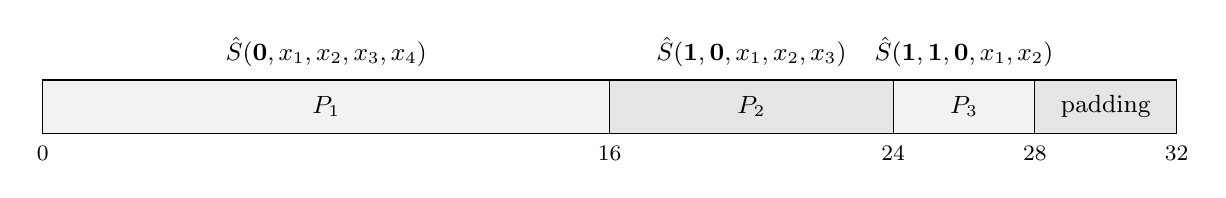
\begin{tikzpicture}[scale=0.45, every node/.style={font=\small}]
    \fill[gray!10] (0,0) rectangle (16,1.5);
    \fill[gray!20] (16,0) rectangle (24,1.5);
    \fill[gray!10] (24,0) rectangle (28,1.5);
    \fill[gray!20] (28,0) rectangle (32,1.5);

    \draw[black] (0,0) rectangle (32,1.5);
    \draw[black] (16,0) -- (16,1.5);
    \draw[black] (24,0) -- (24,1.5);
    \draw[black] (28,0) -- (28,1.5);

    \node at (8,0.75) {$P_1$};
    \node at (20,0.75) {$P_2$};
    \node at (26,0.75) {$P_3$};
    \node at (30,0.75) {padding};

    \node[below] at (0,-0.1) {\footnotesize 0};
    \node[below] at (16,-0.1) {\footnotesize 16};
    \node[below] at (24,-0.1) {\footnotesize 24};
    \node[below] at (28,-0.1) {\footnotesize 28};
    \node[below] at (32,-0.1) {\footnotesize 32};

    % Selector annotations above each section
    \node[above] at (8,1.6) {$\hat{S}({\mathbf{0}}, x_1, x_2, x_3, x_4)$};
    \node[above] at (20,1.6) {$\hat{S}({\mathbf{1}}, {\mathbf{0}}, x_1, x_2, x_3)$};
    \node[above] at (26,1.6) {$\hat{S}({\mathbf{1}}, {\mathbf{1}}, {\mathbf{0}}, x_1, x_2)$};
\end{tikzpicture}
\caption{Simple stacking of $P_1, P_2, P_3$ into a single vector $S$}
\label{fig:stacking}
\end{figure}

\subsection{Tables}\label{sec:table-sizes}

The execution trace is split across three \textit{tables}: \textsc{execution}, \textsc{extension}, and \textsc{poseidon}. Each table $T$ is a matrix of base-field elements, with a variable power-of-two height $2^{h_T}$, and a fixed number of columns $n_\text{column}^T = n_\text{shift}^T + n_\text{flat}^T$. Each column $\hat{\textsf{col}}^T_i$ ($i \in [0, n_\text{column}^T)$) is interpreted as a multilinear polynomial in ${h_T}$ variables.

Each VM cycle corresponds to a row of the $\textsc{EXECUTION}$, each poseidon precompile call corresponds to a row of the $\textsc{POSEIDON}$, and each extension precompile call with a size parameter of $n$ (see TODO) corresponds to a row of the $\textsc{EXTENSION}$ table.

We restrict their maximal heights, to ensure logup multiplicites never overflow modulo $p$:

\begin{center}
\begin{tabular}{lc}
\toprule
Table & Max rows \\
\midrule
\textsc{EXECUTION} & $2^{25}$ \\
\textsc{EXTENSION} & $2^{21}$ \\
\textsc{POSEIDON} & $2^{21}$ \\
\bottomrule
\end{tabular}
\end{center}

\subsection{Buses}\label{sec:Bus: interractions between table via logup-GKR}


In order for the tables (Section~\ref{sec:table-sizes}) to exchange data, we use a \emph{bus}: a global channel in which tables may \textsc{Push} or \textsc{Pull} tuples of $\textsf{bus\_width} = 16$ field elements $\Fq$. We enforce the following property: \textit{every tuple is pulled exactly as many times as it is pushed}.

\subsubsection{Different types of interaction}

Every interaction is a tuple of $\textsf{bus\_width} = 16$ field elements with a fixed shape:
$$\sigma = \big(\,\underbrace{d_0,\ \dots,\ d_{N-1}}_{\text{data}},\quad \underbrace{0,\ \dots,\ 0}_{\text{padding}},\quad \textsf{domain\_sep}\,\big),$$

associated to a \emph{multiplicity}: a value $m \in \Fp$ counting the number of times that tuple is pushed (or pulled). The bus should be balanced: for every $\sigma$, the sums of all its \emph{push} multiplicities must equal the sum of all its \emph{pull} multiplicities.

The $N \le 15$ \emph{data} entries fill the low slots, the last slot always holds the \emph{domain separator} $\textsf{domain\_sep}$, and the slots in between are zero.



There are 4 different types of interactions:

\textbf{Memory:} Each memory fetch corresponds to a data pair $(\textsf{value}, \textsf{address})$, tagged with the domain separator $\textsf{memory\_sep} = 1$.

\textbf{Bytecode:} Each instruction fetch is the data tuple $(\textsf{instr}_0, \dots, \textsf{instr}_{11}, \textsf{pc})$, tagged with the domain separator $\textsf{bytecode\_sep} = 2$.

\textbf{Poseidon:} Each \textsc{POSEIDON} precompile call corresponds to a data tuple $(\nu_A, \nu_B, \nu_C)$ of its three memory pointers, tagged with a non-constant domain separator, that encodes some additional infomration (compression / permutation etc.), but which is an odd value $\ge 3$.

\textbf{Extension} Each \textsc{EXTENSION} precompile call corresponds to a data tuple $(\nu_A, \nu_B, \nu_C)$ of its three memory pointers, tagged with a non-constant domain separator, that encodes some additional infomration (dot\_product / add / eq etc.), but which is a a multiple of $4$.

\begin{center}
\begin{tabular}{lll}
\toprule
Kind & data entries & $\textsf{domain\_sep}$ \\
\midrule
Memory                   & $(\textsf{value},\ \textsf{address})$  & $\textsf{memory\_sep} = 1$ \\
Bytecode                 & $(\textsf{instr}_0,\ \dots,\ \textsf{instr}_{11},\ \textsf{pc})$ & $\textsf{bytecode\_sep} = 2$ \\
Poseidon     & $(\nu_A,\ \nu_B,\ \nu_C)$ & odd, $\ge 3$ \\
Extension & $(\nu_A,\ \nu_B,\ \nu_C)$ & multiple of $4$ \\
\bottomrule
\end{tabular}
\end{center}


A table $T$ may \textsc{Push} or \textsc{Pull} various tuples to the common bus.


\subsubsection{Balanced bus proved via logup}

\paragraph{Hashing tuples to a single field element.} For some $\vec\beta = (\beta_1, \ldots, \beta_\ell) \in \Fq^\ell$ sampled uniformly at random, we define:
\[
h_{\vec\beta}(\sigma) \;=\; \sum_{i=0}^{\textsf{bus\_width} - 1} \sigma_i \cdot \hat{eq}\big(\vec\beta,\, [i]_{01}\big) \;=\; \hat{\sigma}(\vec\beta).
\]
By Lemma~\ref{lem:sz} applied to the (non-zero) multilinear polynomial $\hat\sigma - \hat{\sigma'}$ in $\ell$ variables, two distinct tuples collide with probability at most $\ell/q$.

\paragraph{Bus balance as a rational identity.} Enumerate the bus interactions across all tables as a list of pairs $(\sigma_k, m_k)_{1 \leq k \leq K}$, where $\sigma_k \in \Fp^{\textsf{bus\_width}}$ is the pushed (or pulled) tuple data and $m_k \in \Fp$ is its signed multiplicity (positive for \textsc{Push}, negative for \textsc{Pull}) (where we naturally embedd the integers $(-p, p)$ into $\Fp$). Assume that, for every tuple $\sigma$, both the total pushes and the total pulls of $\sigma$ are strictly less than $p$. Then the bus is balanced if and only if, for every $\sigma$, $\sum_{k \,:\, \sigma_k = \sigma} m_k = 0$, which, for $\vec\beta \overset{\$}{\leftarrow} \Fq^\ell$ and $\gamma \overset{\$}{\leftarrow} \Fq$, is equivalent up to completeness error $K / q$ and soundness error $K \ell / q$ to:
\[
\sum_{k=1}^{K} \frac{m_k}{\gamma - h_{\vec\beta}(\sigma_k)} \;=\; 0.
\]

\begin{proof}
(Inspired by \href{https://github.com/openvm-org/stark-backend/blob/main/docs/Soundness_of_Interactions_via_LogUp.pdf}{Soundness of Interactions via LogUp})
Define the $\Fp$-valued multiset $M(\sigma) = \sum_{k \,:\, \sigma_k = \sigma} m_k$, with support $S = \{\sigma : M(\sigma) \neq 0\}$, of size $s = |S|$. The bus is balanced iff $S = \emptyset$.

\emph{Completeness.} If $S = \emptyset$, then $M(\sigma) = 0$ for every $\sigma$, so the rational sum is identically zero wherever it is defined. The sum is undefined when $\gamma$ coincides with some pole $h_{\vec\beta}(\sigma_k)$, which over uniform $\gamma$ happens with probability at most $K/q$:  the protocol's \emph{completeness error}.

\emph{Soundness.} Suppose $S \neq \emptyset$, and define
\[
N(\vec\beta, \gamma) \;:=\; \sum_{\sigma \in S} M(\sigma) \prod_{\sigma' \in S \setminus \{\sigma\}}\!\big(\gamma - h_{\vec\beta}(\sigma')\big), \qquad Q(\vec\beta, \gamma) \;:=\; \prod_{\sigma \in S}\!\big(\gamma - h_{\vec\beta}(\sigma)\big).
\]
Over a common denominator, the rational sum equals $N/Q$. Verifier acceptance requires this fraction to be defined and equal to zero, hence forces $N(\vec\beta, \gamma) = 0$.

\emph{Total degree of $N$.} The degree of $N$, interpreted as multivariable polynomial in $\gamma$ and $\vec\beta$, is at most $(s-1)\ell \leq K \ell$.

\emph{Non-vanishing of $N$.} Pick any $\sigma^\star \in S$ (so $M(\sigma^\star) \neq 0$). To show $N$ is not the zero polynomial in $\Fq[\vec\beta, \gamma]$, substitute the variable $\gamma$ by the polynomial $h_{\vec\beta}(\sigma^\star) \in \Fq[\vec\beta]$. If $N$ were the zero polynomial its image would also be zero. For every $\sigma \in S$ with $\sigma \neq \sigma^\star$, the product $\prod_{\sigma' \in S \setminus \{\sigma\}}$ contains the factor $\gamma - h_{\vec\beta}(\sigma^\star)$ (since $\sigma^\star \in S \setminus \{\sigma\}$), which the substitution sends to $0$; only the $\sigma = \sigma^\star$ summand survives, giving
\[
N\big(\vec\beta,\, h_{\vec\beta}(\sigma^\star)\big) \;=\; M(\sigma^\star) \prod_{\sigma' \in S \setminus \{\sigma^\star\}} (\hat\sigma^\star - \hat\sigma')(\vec\beta) \;\in\; \Fq[\vec\beta].
\]
Each factor in this product is the MLE of the non-zero vector $\sigma^\star - \sigma' \in \Fp^{\textsf{bus\_width}}$, hence a non-zero polynomial in $\vec\beta$. Given that $M(\sigma^\star) \neq 0$, $N$ is non-zero in $\Fq[\vec\beta, \gamma]$.

By Lemma~\ref{lem:sz},
\[
\Pr_{\vec\beta, \gamma}[N(\vec\beta, \gamma) = 0] \;\leq\; K\,\ell/q. \qedhere
\]
\end{proof}


\subsection{AIR constraints}

Every table $T$ has a list of $n^\text{constraints}_T$ AIR (Algebraic Intermediate Representation) constraints. Each AIR constraint $C_k^T$ ($k \in [0, n_\text{constraints}^T)$) is a multivariate polynomial in $n_\text{column}^T + n_\text{shift}^T$ variables: one variable per column (taking its row-$r$ value $\textsf{col}^T_i(r)$ as input), plus one variable per shifted column (taking $\textsf{shift}(\textsf{col}^T_j)[r]$ as input). The constraint is respected by the table's trace if, for every row $r \in [0, 2^{h_T})$,
$$
C_k^T\big(\textsf{col}^T_0(r), \ldots, \textsf{col}^T_{n_\text{column}^T-1}(r),\ \textsf{shift}(\textsf{col}^T_0)[r], \ldots, \textsf{shift}(\textsf{col}^T_{n_\text{shift}^T-1})[r]\big) = 0.
$$

\subsubsection{ZeroCheck: Proving AIR constraints via sumcheck}

For each table $T$, we want to convince the verifier that every constraint $C_k^T$ vanishes on every row of the trace. We proceed in three steps.

\textbf{Batching.} The verifier samples $\alpha \in \Fq$ and we form the batched constraint
\[
H_T \;:=\; \sum_{k=0}^{n_\text{constraints}^T - 1} \alpha^k\, C_k^T,
\]
a polynomial in the same $n_\text{column}^T + n_\text{shift}^T$ variables as each $C_k^T$.

\emph{Completeness}: if every $C_k^T$ vanishes on every row, so does $H_T$.

\emph{Soundness}: if some $C_k^T$ fails to vanish at some row $\vec b^\star$, then $\alpha \mapsto H_T(\vec b^\star)$, then so does $H_T$, except with soudness error $n_\text{constraints}^T/q$ via Schwartz-Zippel (lemma \ref{lem:sz}).

\textbf{Zerocheck.} Let $f_T \in \Fq^{2^{h_T}}$ be the vector whose $\vec b$-th coordinate is
\[
f_T(\vec b) \;:=\; H_T\big(\hat{\textsf{col}}^T_0(\vec b), \ldots, \hat{\textsf{col}}^T_{n_\text{column}^T-1}(\vec b), \overset{\scriptscriptstyle\wedge}{\textsf{shift}}(\textsf{col}^T_0)(\vec b), \ldots, \overset{\scriptscriptstyle\wedge}{\textsf{shift}}(\textsf{col}^T_{n_\text{shift}^T-1})(\vec b)\big),
\]
so the claim is $f_T \equiv 0$. The verifier samples $\vec r \in \Fq^{h_T}$. By Lemma~\ref{lem:sz} applied to the multilinear polynomial (in $h_T$ variables) $\hat{f}_T$, with soundness error $h_T / q$ it suffices to prove that $\hat{f}_T(\vec r) = 0$, i.e.,
\[
\sum_{\vec b \in \{0,1\}^{h_T}} \hat{eq}(\vec b, \vec r) \cdot f_T(\vec b) \;=\; 0.
\]

\textbf{Sumcheck.} Run the standard sumcheck protocol \cite{sumcheck} on the sum above. After $h_T$ rounds with challenges $\vec\beta \in \Fq^{h_T}$, the verifier must check the summand at $\vec b = \vec\beta$: $\hat{eq}(\vec\beta, \vec r)$ is computed directly, and the column and shifted-column evaluations are claimed by the prover and verified as described in Section~\ref{sec:stacking}.

\subsubsection{Batching many ZeroChecks together}

Instead of running the zerocheck above individually for each table, we merge them into a single \emph{back-loaded} sumcheck of $h_{\max} := \max_T h_T$ rounds, using a shared random challenge $\vec r \in \Fq^{h_{\max}}$. For each table $T$, let $\vec r_T \in \Fq^{h_T}$ be the suffix of $\vec r$ of length $h_T$, write $\vec X_{\geq k} := (X_k, \ldots, X_{h_{\max} - 1})$, and define $G_T \in \Fq[X_0, \ldots, X_{h_{\max}-1}]$ by
\[
G_T(\vec X) \;:=\; \Big(\textstyle\prod_{i < h_{\max} - h_T} X_i\Big) \cdot \hat{eq}\big(\vec X_{\geq h_{\max} - h_T},\, \vec r_T\big) \cdot f_T\big(\vec X_{\geq h_{\max} - h_T}\big).
\]

The verifier samples $\lambda \in \Fq$. Enumerating the three tables as $T \in \{\textsc{EXECUTION}, \textsc{EXTENSION}, \textsc{POSEIDON}\}$ with indices $i_T \in \{0, 1, 2\}$, we run a single sumcheck claiming
\[
\sum_{\vec b \in \{0, 1\}^{h_{\max}}} \sum_T \lambda^{i_T}\, G_T(\vec b) \;=\; 0,
\]
which is equivalent, up to soundness error $2/q$ over $\lambda$ from Lemma~\ref{lem:sz}, to the conjunction of the three per-table zerocheck claims.

\subsection{Execution table}


\subsubsection{Columns}

\fbox{At each cycle, we commit to 20 (base) field elements:}

\begin{itemize}
    \item \textbf{pc} (program counter)
    \item \textbf{fp} (frame pointer)
    % \item jump (non zero when a jump occurs)
    \item $\text{addr}_A$, $\text{addr}_B$, $\text{addr}_C$
    \item $\text{value}_A = \textbf{m}[\text{addr}_A]$, $\text{value}_B = \textbf{m}[\text{addr}_B]$, $\text{value}_C = \textbf{m}[\text{addr}_C]$
    \item 12 field elements describing the instruction being executed (see below)
\end{itemize}


\subsubsection{Instruction Encoding}

Each instruction is described by 12 field elements ($\Fp$):

\begin{itemize}
    \item 3 operands: $\text{operand}_A$, $\text{operand}_B$, $\text{operand}_C$
    \item 5 flags ($\in \{0, 1\}$): $\text{flag}_A$, $\text{flag}_B$, $\text{flag}_C$, $\text{flag}^{C}_\textbf{fp}$, $\text{flag}^{AB}_\textbf{fp}$
    \item 3 opcode flags: MUL ($\in \{0, 1\}$), JUMP ($\in \{0, 1\}$), AUX ($\in \{0, 1, 2\}$) (AUX handles both ADD and DEREF)
    \item PRECOMPILE\_DATA
\end{itemize}

$\text{flag}^{AB}_\textbf{fp}$ is only used by precompile instructions; for ADD, MUL, DEREF, and JUMP it is always 0.


\subsubsection{AIR transition constraints}

\fbox{We use transition constraints of degree 5.}

\vspace{5mm}

We define the following values:
\begin{itemize}
    \item $\nu_A = \text{flag}_A \cdot \text{operand}_A + (1 - \text{flag}_A - \text{flag}^{AB}_\textbf{fp}) \cdot \text{value}_A + \text{flag}^{AB}_\textbf{fp} \cdot (\textbf{fp} + \alpha)$ 
    \item $\nu_B = \text{flag}_B \cdot \text{operand}_B + (1 - \text{flag}_B - \text{flag}^{AB}_\textbf{fp}) \cdot \text{value}_B + \text{flag}^{AB}_\textbf{fp} \cdot (\textbf{fp} + \beta)$
    \item $\nu_C = \text{flag}_C \cdot \text{operand}_C + (1 - \text{flag}_C - \text{flag}_\textbf{fp}) \cdot \text{value}_C + \text{flag}_\textbf{fp} \cdot (\textbf{fp} + \gamma)$
\end{itemize}


With the associated constraints:
\begin{itemize}
    \item $(1 - \text{flag}_A - \text{flag}^{AB}_\textbf{fp}) \cdot (\text{address}_A - (\textbf{fp} + \text{operand}_A)) = 0$
    \item $(1 - \text{flag}_B - \text{flag}^{AB}_\textbf{fp}) \cdot (\text{address}_B - (\textbf{fp} + \text{operand}_B)) = 0$
    \item $(1 - \text{flag}_C - \text{flag}^{C}_\textbf{fp}) \cdot (\text{address}_C - (\textbf{fp} + \text{operand}_C)) = 0$
\end{itemize}

\vspace{3mm}\centerline{\rule{10cm}{0.4pt}}\vspace{5mm}

Let $P_0, P_1, P_2$ be the Lagrange basis polynomials at points $0, 1, 2$. Explicitely:

$$P_0(x) = (x-1)\cdot(x-2) / 2 \hspace{10mm} P_1(x) = x \cdot (2-x) \hspace{10mm} P_2(x) = x \cdot (x-1) / 2$$

We define the following values:

\begin{itemize}
    \item ADD = $P_1(\text{AUX})$
    \item DEREF = $P_2(\text{AUX})$
    \item IS\_PRECOMPILE = $1 - (\text{ADD} + \text{MUL} + \text{DEREF} + \text{JUMP})$
\end{itemize}

IS\_PRECOMPILE is used a "bus selector" (see \ref{buses}).

\vspace{3mm}\centerline{\rule{10cm}{0.4pt}}\vspace{5mm}

PRECOMPILE\_DATA encodes the precompile being called, and the parameters of the call:
\begin{itemize}
    \item No precompile $\rightarrow$ PRECOMPILE\_DATA $= 0$
    \item Poseidon precompile $\rightarrow$ PRECOMPILE\_DATA $= 1$
    \item Extension op precompile $\rightarrow$ PRECOMPILE\_DATA $= 2 \cdot \texttt{be} + 4 \cdot \texttt{flag\_add} + 8 \cdot \texttt{flag\_mul} + 16 \cdot \texttt{flag\_eq} + 32 \cdot N$ \hfill ($N$ = length)
\end{itemize}

\vspace{3mm}\centerline{\rule{10cm}{0.4pt}}\vspace{5mm}

For addition, set AUX $= 1$.
\begin{itemize}
    \item $\text{ADD} \cdot(\nu_B - (\nu_A + \nu_C)) = 0$
\end{itemize}


\vspace{3mm}\centerline{\rule{10cm}{0.4pt}}\vspace{5mm}

For multiplication, set MUL $= 1$.
\begin{itemize}
    \item $\text{MUL} \cdot(\nu_B - \nu_A \cdot \nu_C) = 0$
\end{itemize}

\vspace{3mm}\centerline{\rule{10cm}{0.4pt}}\vspace{5mm}

For DEREF instructions, set AUX $= 2$, $\text{flag}_A = 0$, $\text{flag}_B = 1$ and $\text{flag}_C$ / $\text{flag}^{C}_\textbf{fp}$ according to whether the third operand is an immediate value, a memory read, or fp-relative.

The relation $\textbf{m}[\textbf{m}[\textbf{fp} + \alpha] + \beta] = \nu_C$ is then captured by:

\begin{itemize}
    \item $\text{DEREF} \cdot (\text{addr}_B - (\text{value}_A + \text{operand}_B)) = 0$
    \item $\text{DEREF} \cdot (\text{value}_B - \nu_C) = 0$
\end{itemize}

\vspace{3mm}\centerline{\rule{10cm}{0.4pt}}\vspace{5mm}

For (conditional) jumps, set JUMP = 1, with the following constraints, using $J = \text{JUMP} \cdot \nu_A$:
\begin{itemize}
    \item $J \cdot (1 - \nu_A) = 0$
    \item $J \cdot ( \text{next(\textbf{pc})} - \nu_B) = 0$
    \item $J \cdot ( \text{next(fp)} - \nu_C) = 0$
    \item $(1 - J) \cdot ( \text{next(\textbf{pc})} - (\text{\textbf{pc}} + 1)) = 0$
    \item $(1 - J) \cdot (\text{next(fp)} - \textbf{fp}) = 0$
\end{itemize}

Note: the constraint $J \cdot (1 - \nu_A) = 0$ could be removed, as long as it's correctly enforced in the bytecode.

\vspace{3mm}

TODO: Verify and (formally) prove soundness.

\subsection{Poseidon table}

Poseidon \cite{poseidon1} is a permutation of $\Fp^{16}$. The table runs this permutation once per row, and the final part of the row, which is exposed to memory via lookup, is a function of a compile-time bit $\texttt{flag\_permute}$: we perform either a $16 \to 8$ \emph{compression} or a $16 \to 16$ \emph{permutation}.

The execution table hands the precompile three pointers $\nu_A$, $\nu_B$, $\nu_C$ over the precompile bus, and the precompile fetches the two input halves
$$\texttt{left} = \textbf{m}[\nu_A..\nu_A + 8], \qquad \texttt{right} = \textbf{m}[\nu_B..\nu_B + 8].$$
Write $s = \text{poseidon}(\texttt{left} \;\|\; \texttt{right}) \in \Fp^{16}$ for the raw permutation output.

\vspace{2mm}

\paragraph{Compression mode} ($\texttt{flag\_permute} = 0$) Using pairwise addition in $\Fp$:

$$\textbf{m}[\nu_C..\nu_C + 8] = s[0..8] + \texttt{left}$$


\vspace{2mm}

\paragraph{Permute mode} ($\texttt{flag\_permute} = 1$). 

$$\textbf{m}[\nu_C..\nu_C + 16] = s.$$


\vspace{2mm}

The AIR has degree 10 and $\approx 100$ committed columns; a degree-3 variant exists at the cost of $\approx 160$ columns.
\subsubsection{Efficiently verrifying hash-based signatures}\label{efficiently_verrifying_hash-based_signatures}

The following optimizes the $\emph{compression}$ mode, and is incompatible with the $\emph{permutation}$ mode.

Hash-based signatures often rely on tweaks and public parameters (see \cite{ethereum_signatures}).

We present two independent (and composable) optimizations of the poseidon precompile, when both the hash digest and the public parameters are composed of $n = 4$ field elements. We also assume each tweak occupies less than $n$ field elements (in practice 2 is enough).

\vspace{5mm}

\textbf{1. Chopped output}

We introduce a boolean flag $\texttt{flag\_short}$ that signals that only the first $\texttt{n}$ field elements of the output should be written to memory, at $\textbf{m}[\nu_C..\nu_C + \texttt{n}]$ (the remaining $8 - \texttt{n}$ ones are ignored), 

\vspace{5mm}

\textbf{2. Custom first-half of left-input}

We introduce a boolean flag $\texttt{flag\_left}$, alongside a compile-time parameter $\texttt{offset\_left}$:
$$\texttt{left} = \begin{cases} \textbf{m}[\nu_A..\nu_A + 8] & \text{if } \texttt{flag\_left} = 0 \text{ (default)} \\ \textbf{m}[\texttt{offset\_left}..\texttt{offset\_left} + 4] \;\|\; \textbf{m}[\nu_A..\nu_A + 4] & \text{if } \texttt{flag\_left} = 1 \end{cases}$$

\vspace{5mm}

Both optimizations can be implemented (together), at the cost of 4 additional columns, and incrementing the degree of the constraints by 1.

Both flags ($\texttt{flag\_short}$ and $\texttt{flag\_left}$) and the offset ($\texttt{offset\_left}$) can be encoded in a single (compile-time) parameter, as follows:
$$\texttt{AUX} = 1 + 2 \cdot \texttt{flag\_permute} + 4 \cdot \texttt{flag\_short} + 8 \cdot \texttt{flag\_left} + 16 \cdot \texttt{offset\_left} \cdot  \texttt{flag\_left}$$

Soundness of this encoding (encoding multiple data into a single field element requires care, to avoid overflows that would break injectivity):
\begin{itemize}
    \item both flags are asserted to be boolean by the AIR constraints
    \item if $\texttt{flag\_left} = 0$: then $\texttt{offset\_left}$ is unconstrained: but it does not contribute to the encoding $\texttt{AUX}$, and it has no effect in the AIR logic.
    \item if $\texttt{flag\_left} = 1$: then for the lookup into memory $\textbf{m}[\texttt{offset\_left}..\texttt{offset\_left} + 4]$ to be valid, $\texttt{offset\_left}$ must be smaller than the memory size $M \leq 2^{26} < p / 2$. As a result no overflow can occur in the encoding of $\texttt{AUX}$, which is thus injective.
\end{itemize}

\textbf{Conclusion.} Every tuple $(\nu_A, \nu_B, \nu_C, \texttt{AUX})$ pushed by the execution table is faithfully pulled and decoded by the Poseidon table: the recovered triple $(\texttt{flag\_short}, \texttt{flag\_left}, \texttt{offset\_left})$ matches the one used at the call site, with one harmless exception: when $\texttt{flag\_left} = 0$, $\texttt{offset\_left}$ is left unconstrained, but this is inconsequential since it then has no effect at the AIR level.

\subsection{Extension op table}

See \ref{extension_op_instruction} for the instruction specification.

\subsubsection{Trace layout}

Each extension field operation occupies $N$ consecutive rows (one row per element pair). Within a group, rows are ordered from first element to last, but the \texttt{computation} column accumulates backward: the first row holds the full result, the last row holds only the final element's value. Padding rows have all operation flags set to 0 and $\texttt{start} = 1$, $\texttt{len} = 1$.

\vspace{3mm}

\noindent\resizebox{\textwidth}{!}{%
\begin{tabular}{ccccccccccccccc}
\toprule
\multicolumn{14}{c}{29 base field columns (AIR)} & \\
\texttt{be} & \texttt{start} & $\texttt{f}_\texttt{add}$ & $\texttt{f}_\texttt{mul}$ & $\texttt{f}_\texttt{eq}$ & \texttt{len} & $\text{idx}_A$ & $\text{idx}_B$ & $\text{idx}_R$ & $v_A$ \tiny{(5 cols)} & $v_B$ \tiny{(5 cols)} & \texttt{res} \tiny{(5 cols)} & \texttt{comp} \tiny{(5 cols)} & & \texttt{aux} \\
\midrule
\multicolumn{15}{l}{\textit{MUL, BE, $N\!=\!4$ ($\nu_A\!=\!90$, $\nu_B\!=\!211$, $\nu_C\!=\!74$): \quad $\texttt{res} = \sum_{i=0}^{3} \textbf{m}[90\!+\!i] \cdot \textbf{m}[211\!+\!5i..216\!+\!5i]$}} \\[2pt]
1 & 1 & 0 & 1 & 0 & 4 & 90  & 211 & 74 & $\textbf{m}[90..95]$  & $\textbf{m}[211..216]$ & $\textbf{m}[74..79]$ & $e_0\!+\!e_1\!+\!e_2\!+\!e_3$ & & 138 \\
1 & 0 & 0 & 1 & 0 & 3 & 91  & 216 & 74 & $\textbf{m}[91..96]$  & $\textbf{m}[216..221]$ & $\textbf{m}[74..79]$ & $e_1\!+\!e_2\!+\!e_3$       & & 106 \\
1 & 0 & 0 & 1 & 0 & 2 & 92  & 221 & 74 & $\textbf{m}[92..97]$  & $\textbf{m}[221..226]$ & $\textbf{m}[74..79]$ & $e_2\!+\!e_3$               & & 74 \\
1 & 0 & 0 & 1 & 0 & 1 & 93  & 226 & 74 & $\textbf{m}[93..98]$  & $\textbf{m}[226..231]$ & $\textbf{m}[74..79]$ & $e_3$                       & & 42  \\
\midrule
\multicolumn{15}{l}{\textit{ADD, EE, $N\!=\!3$ ($\nu_A\!=\!400$, $\nu_B\!=\!500$, $\nu_C\!=\!300$): \quad $\texttt{res} = \sum_{i=0}^{2} (\textbf{m}[400\!+\!5i..405\!+\!5i] + \textbf{m}[500\!+\!5i..505\!+\!5i])$}} \\[2pt]
0 & 1 & 1 & 0 & 0 & 3 & 400 & 500 & 300 & $\textbf{m}[400..405]$ & $\textbf{m}[500..505]$ & $\textbf{m}[300..305]$ & $e_0\!+\!e_1\!+\!e_2$ & & 100 \\
0 & 0 & 1 & 0 & 0 & 2 & 405 & 505 & 300 & $\textbf{m}[405..410]$ & $\textbf{m}[505..510]$ & $\textbf{m}[300..305]$ & $e_1\!+\!e_2$         & & 68 \\
0 & 0 & 1 & 0 & 0 & 1 & 410 & 510 & 300 & $\textbf{m}[410..415]$ & $\textbf{m}[510..515]$ & $\textbf{m}[300..305]$ & $e_2$                 & & 36 \\
\midrule
\multicolumn{15}{l}{\textit{EQ, EE, $N\!=\!3$ ($\nu_A\!=\!600$, $\nu_B\!=\!700$, $\nu_C\!=\!800$): \quad $\texttt{res} = \prod_{i=0}^{2} [a_i b_i + (1\!-\!a_i)(1\!-\!b_i)]$}} \\[2pt]
0 & 1 & 0 & 0 & 1 & 3 & 600 & 700 & 800 & $\textbf{m}[600..605]$ & $\textbf{m}[700..705]$ & $\textbf{m}[800..805]$ & $e_0 \cdot e_1 \cdot e_2$ & & 112 \\
0 & 0 & 0 & 0 & 1 & 2 & 605 & 705 & 800 & $\textbf{m}[605..610]$ & $\textbf{m}[705..710]$ & $\textbf{m}[800..805]$ & $e_1 \cdot e_2$           & & 80 \\
0 & 0 & 0 & 0 & 1 & 1 & 610 & 710 & 800 & $\textbf{m}[610..615]$ & $\textbf{m}[710..715]$ & $\textbf{m}[800..805]$ & $e_2$                     & & 48 \\
\midrule
\multicolumn{15}{l}{\textit{Padding row}} \\[2pt]
0 & 1 & 0 & 0 & 0 & 1 & 0   & 0   & 0   & $\textbf{m}[0..5]$ & $\textbf{m}[0..5]$ & $\textbf{m}[0..5]$ & 0 & & 32 \\
\bottomrule
\end{tabular}%
}

\vspace{3mm}

Notes: $e_i$ denotes the per-element result (virtual, not a committed column). $v_A$ stores 5 base-field coordinates $\textbf{m}[\text{idx}_A..\text{idx}_A\!+\!5]$; in BE mode only the first coordinate is used, in EE mode all 5 are used. \texttt{aux} is a non-committed bus fingerprinting column, equal to $2 \cdot \texttt{be} + 4 \cdot \texttt{flag\_add} + 8 \cdot \texttt{flag\_mul} + 16 \cdot \texttt{flag\_eq} + 32 \cdot \texttt{len}$ on each row. The bus selector is the virtual column $\texttt{activation\_flag} = \texttt{start} \cdot \texttt{active}$ (not shown; equals \texttt{start} on active rows, 0 on padding).

\subsubsection{Columns}

\fbox{29 columns.}

\vspace{3mm}

All columns are base field ($\Fp$) columns. Extension field values are represented as 5 consecutive base field columns.

\vspace{2mm}

\begin{itemize}
    \item \texttt{be} $\in \{0,1\}$: mode flag (1: base $\times$ extension, 0: extension $\times$ extension)
    \item \texttt{start} $\in \{0,1\}$: group boundary (1 on first row of each group and on padding, 0 elsewhere)
    \item $\texttt{flag\_add}$, $\texttt{flag\_mul}$, $\texttt{flag\_eq}$ $\in \{0,1\}$: operation selectors (exactly one is 1 on active rows, all 0 on padding)
    \item \texttt{len}: countdown from $N$ to 1 within each group (1 on padding)
    \item $\text{idx}_A$, $\text{idx}_B$, $\text{idx}_R$: memory addresses
    \item $v_A$ (5 cols). In BE mode only the first coordinate is used; in EE mode all 5.
    \item $v_B$ (5 cols)
    \item \texttt{res} (5 cols) (same on every row of a group)
    \item \texttt{comp} (5 cols): running accumulation; equals \texttt{res} on \texttt{start} rows
\end{itemize}

\textbf{Non-committed columns} (used for bus interaction):
\begin{itemize}
    \item $\texttt{activation\_flag} = \texttt{start} \cdot \texttt{active}$: bus selector (1 on first row of each active group, 0 elsewhere)
    \item \texttt{aux} $= 2 \cdot \texttt{be} + 4 \cdot \texttt{flag\_add} + 8 \cdot \texttt{flag\_mul} + 16 \cdot \texttt{flag\_eq} + 32 \cdot \texttt{len}$
\end{itemize}

\subsubsection{Memory lookups}
\begin{itemize}
    \item $v_A = \textbf{m}[\text{idx}_A..+5]$
    \item $v_B = \textbf{m}[\text{idx}_B..+5]$
    \item $\texttt{res} = \textbf{m}[\text{idx}_R..+5]$
\end{itemize}

\subsubsection{Bus interaction}
On rows where $\texttt{activation\_flag} = 1$ (i.e.\ $\texttt{start} = 1$ and $\texttt{active} = 1$), the table \textsc{Pulls} the tuple $(\texttt{aux}, \text{idx}_A, \text{idx}_B, \text{idx}_R)$ from the precompile bus. The execution table \textsc{Pushes} a matching tuple for each EXTENSION\_OP instruction.


The $\texttt{aux}$ encoding ensures both the mode and the length are bound to the bus data. Since $\texttt{be}$, $\texttt{flag\_add}$, $\texttt{flag\_mul}$, and $\texttt{flag\_eq}$ are constrained to be boolean, and since the length is constrained to be $\leq 2^{20}$ (by Lemma~\ref{lem:len-bound}), no overflow can occur modulo $p$ and the $\texttt{aux}$ value is unique for each combination of parameters, which enforces that all values of PRECOMPILE\_DATA sent by the execution table are correctly received by the extension\_op table.


\subsubsection{AIR constraints}

\fbox{Degree 6.}

\vspace{2mm}

\textbf{Value selection:} In BE mode, $v_A$ is treated as a base field element (only the first of its 5 coordinates matters); in EE mode all 5 coordinates are used. Formally, for $k = 1, \dots, 4$: $v_A[k]$ is multiplied by $(1 - \texttt{be})$ in the constraints, so only $v_A[0]$ survives in BE mode.

Let $\texttt{active} = \texttt{flag\_add} + \texttt{flag\_mul} + \texttt{flag\_eq}$ (1 on active rows, 0 on padding), and define the per-element results (virtual):
\begin{align*}
    e_\text{add} &= v_A + v_B \\
    e_\text{mul} &= v_A \cdot v_B \\
    e_\text{peq} &= v_A \cdot v_B + (1 - v_A)(1 - v_B)
\end{align*}

Let $\texttt{comp\_tail} = \text{next}(\texttt{comp}) \cdot (1 - \text{next}(\texttt{start}))$ (zero when the next row is a new group).

\vspace{2mm}

\textbf{Boolean constraints:}
\begin{enumerate}
    \item $\texttt{be} \cdot (1 - \texttt{be}) = 0$
    \item $\texttt{start} \cdot (1 - \texttt{start}) = 0$
    \item $\texttt{flag\_add} \cdot (1 - \texttt{flag\_add}) = 0$
    \item $\texttt{flag\_mul} \cdot (1 - \texttt{flag\_mul}) = 0$
    \item $\texttt{flag\_eq} \cdot (1 - \texttt{flag\_eq}) = 0$
\end{enumerate}

\textbf{Accumulation constraint:}
\begin{enumerate}
    \setcounter{enumi}{5}
    \item $\texttt{f}_\texttt{add} \cdot (\texttt{comp} - e_\text{add} - \texttt{comp\_tail}) = 0$ \hfill (additive ADD)
    \item $\texttt{f}_\texttt{mul} \cdot (\texttt{comp} - e_\text{mul} - \texttt{comp\_tail}) = 0$ \hfill (additive MUL)
    \item $\texttt{f}_\texttt{peq} \cdot (\texttt{comp} - e_\text{peq} \cdot (\texttt{comp\_tail} + \text{next}(\texttt{start}))) = 0$ \hfill (multiplicative EQ)
\end{enumerate}

\vspace{2mm}

\textbf{Result constraint:}
\begin{enumerate}
    \setcounter{enumi}{8}
    \item $\texttt{start} \cdot (\texttt{comp} - \texttt{res}) = 0$ \hfill (on start rows, computation equals result)
\end{enumerate}

\textbf{Intra-group consistency:}
\begin{enumerate}
    \setcounter{enumi}{9}
    \item $(1 - \text{next}(\texttt{start})) \cdot (\texttt{len} - \text{next}(\texttt{len}) - 1) = 0$ \hfill (len countdown)
    \item $(1 - \text{next}(\texttt{start})) \cdot (\texttt{be} - \text{next}(\texttt{be})) = 0$ \hfill (mode consistent)
    \item $(1 - \text{next}(\texttt{start})) \cdot (\texttt{f}_\texttt{add} - \text{next}(\texttt{f}_\texttt{add})) = 0$
    \item $(1 - \text{next}(\texttt{start})) \cdot (\texttt{f}_\texttt{mul} - \text{next}(\texttt{f}_\texttt{mul})) = 0$
    \item $(1 - \text{next}(\texttt{start})) \cdot (\texttt{f}_\texttt{peq} - \text{next}(\texttt{f}_\texttt{peq})) = 0$
    \item $(1 - \text{next}(\texttt{start})) \cdot (\text{next}(\text{idx}_A) - \text{idx}_A - (\texttt{be} + (1 - \texttt{be}) \cdot 5)) = 0$
    \item $(1 - \text{next}(\texttt{start})) \cdot (\text{next}(\text{idx}_B) - \text{idx}_B - 5) = 0$
\end{enumerate}

\textbf{Boundary:}
\begin{enumerate}
    \setcounter{enumi}{16}
    \item $\text{next}(\texttt{start}) \cdot (\texttt{len} - 1) = 0$ \hfill (when next row is a group start, current len must be 1)
\end{enumerate}

\vspace{5mm}

\begin{lemma}\label{lem:len-bound}
On every row $r$ of the dot product table, $\texttt{len}_r \leq H - r$ (as an integer in $\{0, \dots, p-1\}$), where $H \leq 2^{21}$ is the table height. In particular, $\texttt{len}_r \leq H$.
\end{lemma}

\begin{proof}
By backward induction on $r$, from $r = H - 1$ down to $r = 0$.

\vspace{2mm}

\textbf{Base case ($r = H - 1$):} On the wrapping pair (row $H\!-\!1$ paired with itself, see Section~\ref{sec:air-eval}), $\text{next}(x) = x$ for every column $x$. Constraint~10 becomes $(1 - \texttt{start}) \cdot (\texttt{len} - \texttt{len} - 1) = -(1 - \texttt{start}) = 0$, forcing $\texttt{start}_{H-1} = 1$. Then constraint~17 becomes $1 \cdot (\texttt{len} - 1) = 0$, giving $\texttt{len}_{H-1} = 1 = H - (H-1)$.

\vspace{2mm}

\textbf{Inductive step ($r < H - 1$):} Assume $\texttt{len}_s \leq H - s$ for all $s > r$. The pair (row $r$, row $r\!+\!1$) gives two cases depending on $\texttt{start}_{r+1} \in \{0,1\}$ (constraint~2):

\begin{itemize}
    \item If $\texttt{start}_{r+1} = 1$: constraint~17 gives $1 \cdot (\texttt{len}_r - 1) = 0$, so $\texttt{len}_r = 1 \leq H - r$.
    \item If $\texttt{start}_{r+1} = 0$: constraint~10 gives $(1 - 0) \cdot (\texttt{len}_r - \texttt{len}_{r+1} - 1) = 0$, so $\texttt{len}_r = \texttt{len}_{r+1} + 1$ in $\Fp$. By induction, $\texttt{len}_{r+1} \leq H - (r+1)$, so $\texttt{len}_{r+1} + 1 \leq H - r$. Since $H - r \leq H \leq 2^{21} < p$, the addition does not overflow modulo $p$, so $\texttt{len}_r = \texttt{len}_{r+1} + 1 \leq H - r$ as integers.
\end{itemize}
\end{proof}

\vspace{3mm}

TODO: Verify and (formally) prove soundness.

\subsection{Data flow between tables / memory}


\begin{lemma}
    Let $a_0, a_1, \ldots, a_{n-1}$ be pairwise distinct poles in $\Fq$, and let $m_0, m_1, \ldots, m_{n-1}$ be an associated list of multiplicities in $\{0, 1, \dots, p - 1\}$. Consider the rational function:
$$P(X) = \sum_{i=0}^{n-1} \frac{m_i}{X - a_i}$$

Except with probability $n/q$, if $P(\alpha) = 0$ for a random $\alpha \in \Fq$, then all multiplicities $m_i = 0$.

\end{lemma}

\subsubsection{Indexed Lookup into Memory}\label{sec:memory-lookup}

We use logup \cite{logup}, in its indexed form, to allow tables to perform lookups into the read-only memory.


\vspace{3mm}

Let $\mathcal{T}$ denote the set of all tables in the system. For each table $T \in \mathcal{T}$ with $H_T$ rows, let $n_T$ denote the number of memory lookups. Each lookup $i < n_T$ consists of an \textbf{index column} $\text{col}_{\text{index},T,i}$ and a \textbf{value column} $\text{col}_{\text{val},T,i}$.

\vspace{3mm}

The rule to enforce is the following:
$$\forall T \in \mathcal{T}, \forall i < n_T, \forall j < H_T: \quad \text{col}_{\text{val},T,i}(j) = \textbf{m}[\text{col}_{\text{index},T,i}(j)]$$

Implicitly, we must also have $\text{col}_{\text{index},T,i}(j) < M$ (the memory size).

\vspace{3mm}

The prover initially commits to a multilinear polynomial $\textit{acc}$, having the same size as the memory, such that (in the honest case) for every $k < M$:
$$\textit{acc}[k] = \sum_{T \in \mathcal{T}} \sum_{i < n_T} \left| \{ j < H_T : \text{col}_{\text{index},T,i}(j) = k \} \right|$$
i.e., $\textit{acc}[k]$ represents the total number of times address $k$ is accessed by the lookups across all tables.

\vspace{3mm}

The verifier sends a random challenge $\alpha \in \Fq$ (TODO quantify soundness error). Let $N = \sum_{T \in \mathcal{T}} n_T \cdot H_T$ be the total number of memory lookups. Assuming $N < p$ (to avoid overflow), the indexed lookup into memory is valid, except with probability $(N + M)/q$, if for a randomly sampled $X \in \Fq$:

$$\sum_{T \in \mathcal{T}} \sum_{i<n_T} \sum_{j<H_T} \frac{1}{X - (\text{col}_{\text{index},T,i}(j) + \alpha \cdot \text{col}_{\text{val},T,i}(j))} = \sum_{k<M} \frac{\textit{acc}(k)}{X - (k + \alpha \cdot \textbf{m}[k])}$$

This can be computed via GKR, as introduced in \cite{logup_gkr}.

\subsubsection{Precompile bus: Data flow between tables}\label{buses}

See OpenVM \cite{openvm}, definition 2.2.2, for more details.

At each cycle when IS\_PRECOMPILE = 1, the execution table \textsc{Push}es $$\sigma = (\text{PRECOMPILE\_DATA}, \nu_A, \nu_B, \nu_C)$$ to the "precompile bus".

In case of Poseidon call, PRECOMPILE\_DATA = 1 and $\nu_A$, $\nu_B$, $\nu_C$ represent the left input address, the right input address, and the output address (3 pointers to a chunk of 8 field elements in memory).

In case of extension op call, PRECOMPILE\_DATA $= 2 \cdot \texttt{be} + 4 \cdot \texttt{flag\_add} + 8 \cdot \texttt{flag\_mul} + 16 \cdot \texttt{flag\_eq} + 32 \cdot N$ encodes the mode, the operation, and the length $N$, and $\nu_A$, $\nu_B$, $\nu_C$ represent the starting address of the first operand, the starting address of the second operand, and the address of the result.

Each such tuple $\sigma$ (counting multiplicity) must be \textsc{Pulled} by one of the precompile tables. Given that the Poseidon table only pulls tuples with PRECOMPILE\_DATA $= 1$, and the extension op table only pulls tuples with PRECOMPILE\_DATA $\geq 32$, the bus is effectively partitioned into two disjoint sub-buses, one for each precompile.

Similarly to the IS\_PRECOMPILE (virtual) column for the execution table, each one of the two precompile tables has a boolean (virtual) column acting as a bus selector, indicating at which rows the table is pulling from the bus (1) or not (0).

\vspace{3mm}

\textbf{Balance rule:} At the end of execution, for each tuple $\sigma$, the number of pushes must equal the number of pulls accross the 3 tables: execution, poseidon, and extension op.

\vspace{5mm}

\textbf{Proving system (logup):}

Let $\mathcal{T}$ denote the set of all tables in the system. Each table $T \in \mathcal{T}$ has $H_T$ rows. The bus interaction of the table $T$ is defined by:
\begin{itemize}
    \item $\text{dir}_{T} \in \{+1, -1\}$: the direction ($+1$ for \textsc{Push}, $-1$ for \textsc{Pull})
    \item $\text{sel}_{T}: [0, H_T) \to \{0, 1\}$: the selector (virtual) column
    \item $\sigma_{T} = (\sigma_0, \ldots, \sigma_{k-1})$: the $k$ data columns
\end{itemize}

\vspace{3mm}

The verifier sends a random challenge $\alpha \in \Fq$. Define the encoding of a tuple $\sigma = (\sigma_0, \ldots, \sigma_{k-1})$ by:
$$\text{encode}(\sigma_0, \ldots, \sigma_{k-1}) = \sum_{i=0}^{k-1} \alpha^{i} \cdot \sigma_i$$

\vspace{3mm}

Except with negligible probability probability (TODO quantify precisely), the bus is balanced if for a randomly sampled $X \in \Fq$:

$$\sum_{T \in \mathcal{T}} \sum_{j=0}^{H_T - 1} \frac{\text{dir}_{T} \cdot \text{sel}_{T}(j)}{X - \text{encode}(\sigma_{T}(j))} = 0$$


\vspace{3mm}

\textit{Overflow constraint:} We must ensure that multiplicities do not overflow modulo $p$. This is enforced by limitting the maximum height of each table.

\vspace{3mm}

As with the indexed lookup into memory, this sum can be computed efficiently via GKR \cite{logup_gkr}. In practice, all logup instances (bus balance and memory lookups) are batched into a single GKR instance, using an addition field element passed to the encoding tuple for domain separation.

\vspace{3mm} TODO: Unified vision in which memory is just another table, and memory accesses are just bus interactions?

A detailled soundness analysis can be found in \href{https://github.com/openvm-org/stark-backend/blob/main/docs/Soundness_of_Interactions_via_LogUp.pdf}{Soundness of Interactions via LogUp}.



\subsection{ISA programming}

\subsubsection{Functions}

\begin{enumerate}
    \item Each function has a deterministic memory footprint: the length of the continuous frame in memory that is allocated for each of the its calls.
    \item At runtime, each time we call our function, we receive via a memory cell a hint pointing to a free range of memory. We then store the current values of \textbf{pc} / \textbf{fp} at the start of this newly allocated frame, alongside the function's arguments, we can then jump, to enter the function bytecode, and modify \textbf{fp} with the hinted value. The intuition here is that the verifier does not care where the new memory frame will be placed (we use a read-only memory, so we cannot overwrite previous frames). In practice, the prover that runs the program would need to keep the value of the allocation pointer "ap", in order to adequately allocate new memory frames, but there is no need to keep track of it from the versifier's perspective.
\end{enumerate}


\begin{figure}[h]
\caption{Memory layout of a function call}
\centering
\includegraphics[scale=0.4]{images/memory_layout.png}
\end{figure}

\subsubsection{Loops}\label{loops}

We suggest to unroll loops when the number of iterations is low, and known at compile time.
The remaining loops are transformed into recursive functions (by the leanISA compiler).

\subsubsection{Range checks}

\fbox{It's possible to check that a memory cell is smaller than $t$ (for $t \leq 2^{16}$) in 3 cycles.}

We denote by \textbf{m}[\textbf{fp} + $x$] the memory cell for which we want to ensure \textbf{m}[\textbf{fp} + $x$] $< t$.
We also denote by \textbf{m}[\textbf{fp} + $i$], \textbf{m}[\textbf{fp} + $j$] and \textbf{m}[\textbf{fp} + $k$] 3 auxiliary memory cells (that have not been used yet).
\begin{enumerate}
    \item \textbf{m}[\textbf{m}[\textbf{fp} + $x$]] = \textbf{m}[\textbf{fp} + $i$] (using DEREF, this ensures \textbf{m}[\textbf{fp} + $x$] $ < M$, the memory size)
    \item \textbf{m}[\textbf{fp} + $x$] + \textbf{m}[\textbf{fp} + $j$] = (t-1) (using ADD, this computes $\textbf{m}[\textbf{fp} + $j$] = t - 1 - $ \textbf{m}[\textbf{fp} + $x$])
        \item \textbf{m}[\textbf{m}[\textbf{fp} + $j$]] = \textbf{m}[\textbf{fp} + $k$] (using DEREF, this ensures $t - 1 - $ \textbf{m}[\textbf{fp} + $x$] $ < M$)
\end{enumerate}

Given $t \leq 2^{16} \leq M$, \textbf{m}[\textbf{fp} + $x$] $ < M$, $t - 1 - $ \textbf{m}[\textbf{fp} + $x$] $< M$, and $M \leq 2^{26} < p / 2$, we have: \textbf{m}[\textbf{fp} + $x$] $ < t$.

Note: From the point of view of the prover running the program, some hints are necessary (filling the values of \textbf{m}[\textbf{fp} + $i$] and \textbf{m}[\textbf{fp} + $k$] must be done at end of execution).

This idea was pointed out by D. Khovratovich, and is an unplanned use of the DEREF instruction.

\begin{exmp}
	Let's say we want to write a function with 2 arguments $x = \textbf{m}$[\textbf{fp} + 2] and $y = \textbf{m}$[\textbf{fp} + 3] ($\textbf{m}$[\textbf{fp} + 0] and $\textbf{m}$[\textbf{fp} + 1] are used, by convention, to store the caller's \textbf{pc} and \textbf{fp}, to return to the previous context at the end of the function), which perform the following:
	
	\begin{enumerate}
		\item assert(x $<$ 10)
		\item z := x*y + 100
		\item assert(z $<$ 1000)
	\end{enumerate}
	
	Which can be compiled to:
	
	\begin{enumerate}
		\item \textbf{m}[\textbf{fp} + 4] = \textbf{m}[\textbf{m}$\big[$\textbf{fp} + 2$\big]$] // check that $x$ is "small"
		\item \textbf{m}[\textbf{fp} + 2] + \textbf{m}[\textbf{fp} + 5] = 9 // compute $9 - x$
		\item \textbf{m}[\textbf{fp} + 6] = \textbf{m}[\textbf{m}$\big[$\textbf{fp} + 5$\big]$] // check that $9 - x$ is "small"
		\item \textbf{m}[\textbf{fp} + 7] = \textbf{m}[\textbf{fp} + 2] * \textbf{m}[\textbf{fp} + 3] // compute $x.y$
		\item \textbf{m}[\textbf{fp} + 8] = \textbf{m}[\textbf{fp} + 7] + 100 // compute $z = x.y + 100$
		\item \textbf{m}[\textbf{fp} + 9] = \textbf{m}[\textbf{m}$\big[$\textbf{fp} + 8$\big]$] // check that $z$ is "small"
		\item \textbf{m}[\textbf{fp} + 8] + \textbf{m}[\textbf{fp} + 10] = 999 // compute $999 - z$
		\item \textbf{m}[\textbf{fp} + 11] = \textbf{m}[\textbf{m}$\big[$\textbf{fp} + 10$\big]$] // check that $999 - z$ is "small"
		\item JUMP with next(\textbf{pc}) = \textbf{m}[\textbf{fp} + 0], next(\textbf{fp}) = \textbf{m}[\textbf{fp} + 1], condition = 1 // return
	\end{enumerate}
	
	 
\end{exmp}


\subsubsection{Switch statements}

Suppose we want a different logic depending on the value $x$ of a given memory cell, where $x$ is known to be $< k$ (if the value $x$ comes from a "hint", don't forget to range-check it).

Each of the $k$ different values leads to a different branch at runtime, represented by a block of code. We want to jump to the correct block of code depending on $x$.
One efficient implementation consists in placing our blocks of code at regular intervals, and to jump to $a + b \cdot x$, where $a$ is the offset of the first block of code (in case $x = 0$), and $b$ is the distance between two consecutive blocks.

Example: During XMSS verification, for each of the $v$ chains, we need to hash a pre-image, a number of times depending on the encoding, but known to be $< w$. Here $k = w$, and the $i$-th block of code we could jump to will execute $i$ times the hash function (unrolled loop).


\section{Signature aggregation}\label{sec:signature-aggregation}


We need to:
\begin{itemize}
     \item \textbf{Aggregate} hash-based signatures (leanXMSS / leanSPHINCS)
    \item \textbf{Merge} those aggregate signatures $\rightarrow$ recursive proof
\end{itemize}

Aggregation and merging are unified in a single program, that attests knowledge of a list of signatures corresponding to a list of (message, publickey) pairs. In the case the consensus: a single message (block hash) is shared by all signers, at a given slot.

\begin{figure}[ht]
\centering
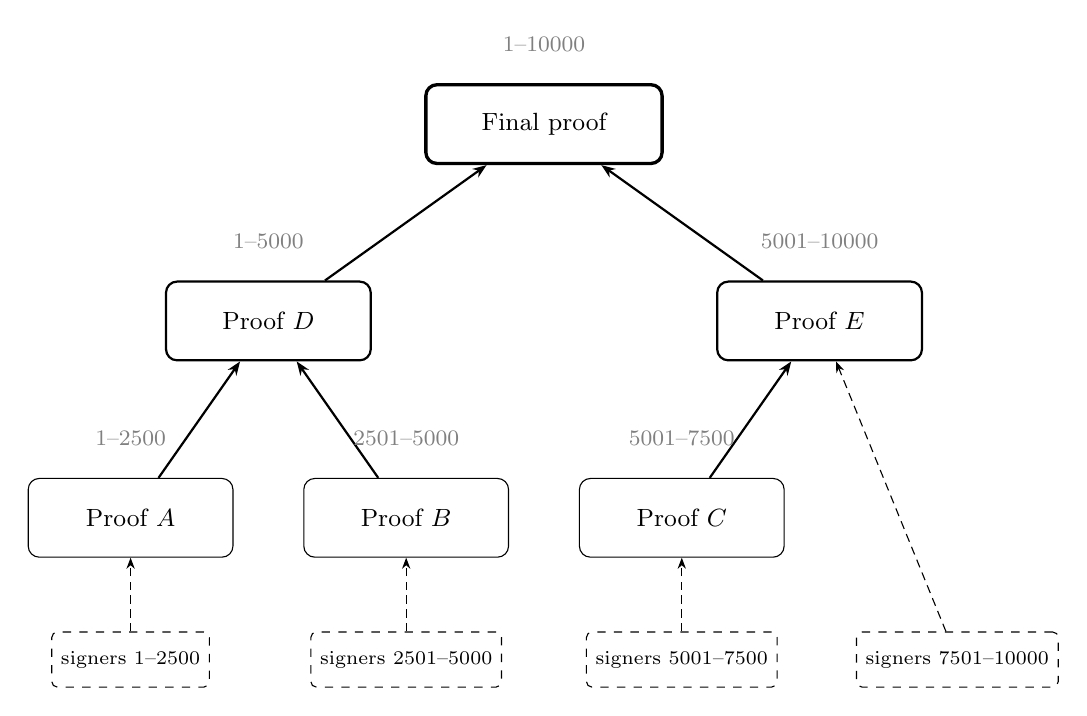
\begin{tikzpicture}[
    proof/.style={draw, rounded corners=4pt, minimum width=2.6cm, minimum height=1cm, align=center, font=\small},
    leaf/.style={proof},
    merge/.style={proof, line width=0.8pt},
    root/.style={proof, minimum width=3cm, line width=1.2pt},
    xmss/.style={draw, dashed, rounded corners=2pt, minimum width=1.6cm, minimum height=0.7cm, align=center, font=\scriptsize},
    attests/.style={font=\footnotesize, text=black!50},
    arr/.style={-{Stealth[length=5pt]}, thick},
    sigarr/.style={-{Stealth[length=4pt]}, densely dashed, thin},
]

% --- XMSS signature blocks (inputs) ---
\node[xmss] (S1) at (0, -1.8) {signers $1$--$2500$};
\node[xmss] (S2) at (3.5, -1.8) {signers $2501$--$5000$};
\node[xmss] (S3) at (7, -1.8) {signers $5001$--$7500$};
\node[xmss] (S4) at (10.5, -1.8) {signers $7501$--$10000$};

% --- Leaf proofs ---
\node[leaf] (L1) at (0, 0) {Proof $A$};
\node[leaf] (L2) at (3.5, 0) {Proof $B$};
\node[leaf] (L3) at (7, 0) {Proof $C$};

% XMSS -> leaf arrows
\draw[sigarr] (S1) -- (L1);
\draw[sigarr] (S2) -- (L2);
\draw[sigarr] (S3) -- (L3);

% --- Middle level ---
\node[merge] (M1) at (1.75, 2.5) {Proof $D$};
\node[merge] (M2) at (8.75, 2.5) {Proof $E$};

% XMSS -> E (direct group)
\draw[sigarr] (S4) -- (M2);

% Recursive arrows: leaves -> middle
\draw[arr] (L1) -- (M1);
\draw[arr] (L2) -- (M1);
\draw[arr] (L3) -- (M2);

% --- Root ---
\node[root] (R) at (5.25, 5) {Final proof};

% Recursive arrows: middle -> root
\draw[arr] (M1) -- (R);
\draw[arr] (M2) -- (R);

% --- Coverage annotations (above each proof) ---
\node[attests, above=8pt of L1] {$1\text{--}2500$};
\node[attests, above=8pt of L2] {$2501\text{--}5000$};
\node[attests, above=8pt of L3] {$5001\text{--}7500$};
\node[attests, above=8pt of M1] {$1\text{--}5000$};
\node[attests, above=8pt of M2] {$5001\text{--}10000$};
\node[attests, above=8pt of R] {$1\text{--}10000$};

\end{tikzpicture}
\caption{Example of recursive aggregation of 10000 XMSS, sharing a common message. (Note: overlapping sets of signers are possible.) }
\label{fig:recursive-aggregation}
\end{figure}


\subsection{Recursive Aggregation}\label{sec:recursive-aggregation}

The recursive aggregation program (see Figure~\ref{fig:recursive-aggregation}) attests that a set of public keys have valid signatures for a given message. It partitions the signers into $n_{\text{rec}} + 1$ sources: one \textbf{direct source} whose XMSS signatures are verified explicitly, and $n_{\text{rec}} \geq 0$ \textbf{recursive sources}, each accompanied by a sub-proof that is recursively verified.

For each recursive source, the program runs the leanVM verifier on the provided sub-proof, confirming that the sub-proof itself is a valid recursive aggregation proof covering the source's signers. When $n_{\text{rec}} = 0$, the program simply verifies all signatures directly.

\subsubsection{Bytecode evaluation claims}\label{sec:bytecode-reduction}

A key subtlety arises from recursion. Every leanVM proof is tied to a specific \emph{bytecode} --- the program that was executed, represented as a multilinear polynomial. In our case, there is a single program (that both contain signature verification and recursion algorithms). The leanVM verification algorithm requires evaluating the bytecode polynomial at a random point.

When the recursive aggregation program verifies a sub-proof, it runs the leanVM verifier \emph{inside} the program. This verification produces a bytecode evaluation claim. For efficiency, rather than checking it inside the program (with a PCS), the claim is forwarded to the public input, to be checked externally.

However, each sub-proof is potentially itself a recursive aggregation, and may have already forwarded its own bytecode claim in the same way. So for each of the $n_{\text{rec}}$ sub-proofs, \textbf{two} bytecode claims arise:

\begin{enumerate}
    \item \textbf{Inner-public-memory claim}: The bytecode claim that the sub-proof forwarded from its own recursive verifications (read from the sub-proof's public input).

    \item \textbf{Inner-proof claim}: The new bytecode claim produced by verifying the sub-proof itself.
\end{enumerate}

After verifying all $n_{\text{rec}}$ sub-proofs, a fresh Fiat--Shamir transcript is initialized and fed with all $2 n_{\text{rec}}$ evaluation points and claimed values. This transcript produces a random linear combination challenge, and the $2 n_{\text{rec}}$ claims are then batched into a single one via sumcheck, yielding a reduced claim. This reduced claim is written to the public input for the next level of recursion.

When $n_{\text{rec}} = 0$ (no recursion), the bytecode claim in the public input is set to zero.


\subsubsection{Signer partitioning}\label{sec:signer-partitioning}

\emph{
In the following, we assume  the message being signed is common to all signers (typically the case at Ethereum's consensus layer), but the scheme can be naturally adapted to distinct messages.}

\vspace{3mm}

Consider an aggregation of $n_{\text{sigs}}$ (distinct) signatures. The $n_{\text{sigs}}$ (distinct) public keys are part of the "public input" in memory. The aggregation program must ensure that each public key is verified by at least one of the $1 + n_{\text{rec}}$ sources (duplications allowed: some public keys may be verified by multiple sources).

Let $n_{\text{dup}}$ be the total number of duplicated public keys across sources, counted with multiplicity. To ensure ensure valid partionning, we use the following algorithm:

\begin{itemize}
    \item Initialize a counter $c \gets 0$.
    \item Initialize a (write-once) array $B$ of size $n_{\text{total}} = n_{\text{sigs}} + n_{\text{dup}}$.
    \item For each source $s$, for each signature index $i \in [0, n_{\text{total}})$ verified by $s$, write $B[i] \gets c$ and increment $c$.
    \item At the end, assert $c = n_{\text{total}}$.
\end{itemize}


\clearpage
\bibliographystyle{IEEEtran}
\bibliography{bibliography}

\end{document}